\begin{figure}[H]
    \centering
    \definecolor{slabblue}{RGB}{100,175,215}
    \definecolor{fieldred}{RGB}{185,45,45}
    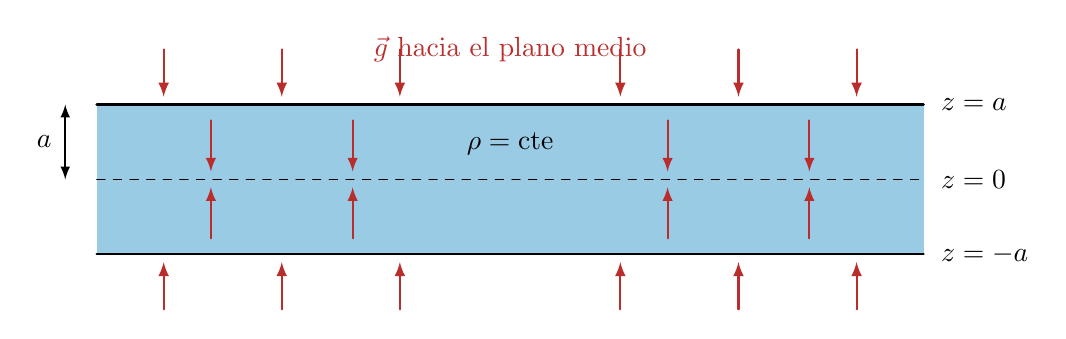
\begin{tikzpicture}[x=1cm,y=1cm,line cap=round,line join=round]
        % Placa infinita vista de canto
        \fill[slabblue!65] (0.75,1.15) rectangle (11.25,3.05);
        \draw[line width=0.9pt] (0.75,1.15) -- (11.25,1.15);
        \draw[line width=0.9pt] (0.75,3.05) -- (11.25,3.05);
        \draw[dashed] (0.75,2.10) -- (11.25,2.10);
        \node[right] at (11.35,3.05) {$z=a$};
        \node[right] at (11.35,2.10) {$z=0$};
        \node[right] at (11.35,1.15) {$z=-a$};
        \node at (6.00,2.55) {$\rho=\mathrm{cte}$};

        % Campo dirigido hacia el plano medio
        \foreach \x in {1.6,3.1,4.6,7.4,8.9,10.4} {
            \draw[fieldred,-latex,line width=0.75pt]
                (\x,3.75) -- (\x,3.15);
            \draw[fieldred,-latex,line width=0.75pt]
                (\x,0.45) -- (\x,1.05);
        }
        \foreach \x in {2.2,4.0,8.0,9.8} {
            \draw[fieldred,-latex,line width=0.70pt]
                (\x,2.85) -- (\x,2.20);
            \draw[fieldred,-latex,line width=0.70pt]
                (\x,1.35) -- (\x,2.00);
        }
        \node[fieldred] at (6.00,3.75) {$\vec g$ hacia el plano medio};

        % Cota de semiespesor
        \draw[latex-latex,line width=0.6pt] (0.35,2.10) -- (0.35,3.05);
        \node[left] at (0.30,2.58) {$a$};
    \end{tikzpicture}
    \caption{Placa autogravitante infinita y dirección de su campo gravitacional.}
\end{figure}